
\title{Sistemi Informativi \\ Laboratorio 5}
\author{
        Catalin Copil
            \and
        Mattia de Stefani
            \and
        Giulio Lovisotto
}
\date{\today}

\documentclass[12pt]{article}
\usepackage{algorithmicx}
\usepackage{algpseudocode}
\usepackage{graphicx}
\usepackage{geometry}

\addtolength{\topmargin}{-.5in}
\begin{document}
\maketitle

\section{Descrizione}
Utilizzeremo la funzione di ranking BM25 con relevance feedback esplicito (lab 5), e applicheremo LSA. Sceglieremo i primi $N$ documenti reperiti (proveremo vari valori di $N$ per trovare quello che garantisce il miglior risultato). Useremo il metodo \texttt{linalg.svd} della libreria \texttt{numpy} per trovare la fattorizzazione della matrice termini-documenti $X$:
\[ X = U \Sigma V^{T}. \]
Dopodiche', considereremo $m$ dimensioni, e proietteremo l'interrogazione $\vec{q}$ sullo spazio a dimensione ridotta usando la formula:
\[ \vec{q}_m = \Sigma^{-1}_m U^{T}_m \vec{q}. \]

Poi computeremo le cosine similarity tra le rappresentazioni degli $N$ documenti nello spazio ridotto (colonne di  $V_m^{T}$) e la query ridotta $\vec{q}_m$. Ordineremo questi $N$ documenti per cosine similarity decrescente, mentre l'ordine di tutti gli altri documenti non verra' alterato, e questi verranno accodati. 

\section{Risultati}

Abbiamo utilizzato i seguenti parametri, $m = 2$, $N=10$. Nel report finale proveremo diverse configurazioni per trovare il miglior risultato. Figura \ref{fig:uno} riporta i valori di map ottenuti.

\begin{figure}[htbp]
\begin{center}
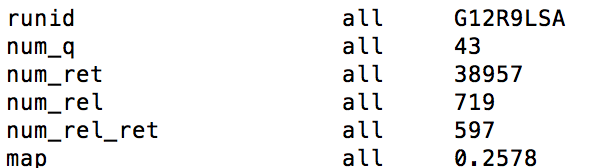
\includegraphics[width=0.9\textwidth]{one.png}
\caption{Map utilizzando LSA.}
\label{fig:uno}
\end{center}
\end{figure}





\bibliographystyle{abbrv}
\bibliography{main}

\end{document}